\documentclass[11pt, letterpaper]{report}
\usepackage{sectsty}
\usepackage[spanish, es-noindentfirst]{babel}
\spanishdecimal{.}
\usepackage[T1]{fontenc}
\usepackage[utf8]{inputenc}

\usepackage{caption} 
\captionsetup[table]{skip=4pt}
\usepackage{setspace}
\setstretch{1.5}
\usepackage{graphicx,microtype} % Required for inserting images
%\usepackage{chngcntr} % sections without chapter numbers
\setcounter{secnumdepth}{3} % Numbered subsubsections
\setcounter{tocdepth}{3} % subsubsections in toc
\setlength{\parskip}{\medskipamount}
\usepackage[colorlinks, linkcolor=blue, urlcolor=blue]{hyperref}
\usepackage{url}
\usepackage[left=3cm, right=3cm, top=2cm, bottom=2cm]{geometry}
\usepackage{minted, verbatim}


\usepackage{unicode-math} 
\usepackage{fontspec}
\setmainfont{Arial}
%\setsansfont{Calibri
\setmonofont{Consolas}
\setmathfont{Cambria Math}

\partfont{\Huge}

\title{\bf\Huge Reducción de datos CCD con IRAF y Python}
\author{Alexis Andrés}
\date{\today}

\usepackage{xcolor}
\usepackage[most]{tcolorbox}
\usepackage{tikz}
\usetikzlibrary{trees}
\usepackage{listings}
\usepackage{textcomp}
\tcbuselibrary{listingsutf8}
\tcbuselibrary{minted}
\usepackage{cprotect}

\usepackage{fvextra}
% Configuración para que mintinline sea en negritas y monoespaciado
\DefineVerbatimEnvironment{Bash}{Verbatim}{formatcom=\bfseries}
\newcommand{\mintbold}[2][]{\mintinline[formatcom=\bfseries,#1]{#2}}

% Python inline
\newcommand{\pybold}[1]{\mintinline[style=friendly,formatcom=\bfseries]{python}{#1}}
\newcommand{\pynorm}[1]{\mintinline[style=friendly]{python}{#1}}

% Bash inline
\newcommand{\bashbold}[1]{\mintinline[style=bw,formatcom=\bfseries]{shell}{#1}}
\newcommand{\norbash}[1]{\mintinline[style=bw]{shell-session}{#1}}

\definecolor{grey}{HTML}{CFCFCF}
\definecolor{light_gray}{rgb}{0.97,0.97,0.97}
\definecolor{mykey}{rgb}{0.117,0.403,0.713}
\definecolor{myorange}{HTML}{BF5B3D}
\definecolor{cellerror}{HTML}{FFDDDD}


\newlength\inwd
\setlength\inwd{2.5em}

\newcounter{ipythcntr}
\renewcommand{\theipythcntr}{\texttt{[\arabic{ipythcntr}]}}

\definecolor{terminalTitle}{RGB}{214,233,246}
\definecolor{terminalColor}{RGB}{238,238,238}
\definecolor{Button1}{RGB}{211,25,25}
\definecolor{Button2}{RGB}{55,124,241}
\definecolor{Button3}{RGB}{253,125,0}

\newtcblisting{terminal}[1][]{
    listing engine=minted,minted style=bw,
    minted language=#1,
    minted options={%
         breaklines,
         obeytabs=true,
         breaksymbolleft=,
         autogobble,
         numbersep=2mm,
         baselinestretch=1},
    coltitle=gray,
    enhanced,
    colback=light_gray,colframe=terminalTitle,listing only, title=\tikz{
        \node[circle,fill=Button1,inner sep=3pt] (c) at (0,0){};
        \node[circle,fill=Button2,inner sep=3pt] (c) at (0.5,0){};
        \node[circle,fill=Button3,inner sep=3pt] (c) at (1,0){};
    },
    every listing/.style={\singlespacing}
    }

\newtcblisting{bash}[1][]{
    boxrule=0.5pt,
    listing engine=minted, minted style=tango,
    minted language=shell-session,
    minted options={%
         breaklines,
         obeytabs=true,
         breaksymbolleft=,
         autogobble,
         numbersep=2mm,
         baselinestretch=1,
         escapeinside=!!},
    enhanced, colback=light_gray,colframe=grey,listing only, 
    %coltext=white!40!black,
    %coltitle=black,
    %title=\tikz { \centering
        %\node[circle,fill=Button1,inner sep=3pt] (c) at (0,0){};
        %\node[circle,fill=Button2,inner sep=3pt] (c) at (0.5,0){};
        %\node[circle,fill=Button3,inner sep=3pt] (c) at (1,0){};
    %} \texttt{#1} ,
    }
    
\newtcblisting{shell}[1][]{
    boxrule=0.5pt,
    breakable,
    listing engine=minted, minted style=bw,
    minted language=shell-session,
    minted options={%
         breaklines,
         obeytabs=true,
         breaksymbolleft=,
         autogobble,
         numbersep=2mm,
         baselinestretch=1,
         escapeinside=!!},
    enhanced, colback=light_gray,colframe=grey,listing only
    }

\newtcblisting{pyin}[1][]{%
  width=\linewidth,
  enhanced,
  colframe=grey,
  boxrule=0.5pt,
  arc=1pt,
  colback=light_gray,
  listing only,
  top=0pt,
  bottom=0pt,
  left=5pt,
  right=5pt,
  breakable,
  overlay={
    \node[
      anchor=north east,
      text width=\inwd,
      font=\footnotesize\ttfamily\color{mykey},
      inner ysep=2mm,
      inner xsep=0pt,
      outer sep=0pt
      ] 
      at (frame.north west)
      {\refstepcounter{ipythcntr}\theipythcntr:};
  }
  listing engine=minted,
  minted style=friendly,
  minted language=python,
  minted options={%
         breaklines,
         obeytabs=true,
         breaksymbolleft=,
         autogobble,
         numbersep=2mm,
         baselinestretch=1},
}

\newtcblisting{pyprint}{
  sharp corners,
  width=\linewidth,
  enhanced,
  coltext=black,
  colframe=white,
  boxrule=0pt,
  colback=white,
  listing only,
  top=-7pt,
  bottom=0pt,
  left=2pt,
  right=1pt,
  overlay={
    \node[
      anchor=north east,
      text width=\inwd,
      font=\footnotesize\ttfamily\color{mykey},
      inner ysep=2mm,
      inner xsep=0pt,
      outer sep=0pt
      ] 
      at (frame.north west)
      {};
  }
  listing engine=minted,
  minted language=pycon,
  minted options={%
         breaklines,
         obeytabs=true,
         breaksymbolleft=,
         autogobble,
         numbersep=2mm,
         baselinestretch=1},
}

\newtcblisting{pyout}[1][\theipythcntr]{
  enlarge left by=0pt,
  width=\linewidth,
  enhanced,
  colframe=white,
  boxrule=0pt,
  colback=white,
  listing only,
  top=0pt,
  bottom=0pt,
  left=7pt,
  right=1pt,
  overlay={
    \node[
      anchor=north east,
      text width=\inwd,
      font=\footnotesize\ttfamily\color{myorange},
      inner ysep=2mm,
      inner xsep=0pt,
      outer sep=0pt
      ] 
      at (frame.north west)
      {\setcounter{ipythcntr}{\value{ipythcntr}}#1:};
  }
  listing engine=minted, 
  minted language=pycon,
  minted options={%
         breaklines,
         obeytabs=true,
         breaksymbolleft=,
         autogobble,
         numbersep=2mm,
         baselinestretch=1},
}

\newtcblisting{pyerror}{
  sharp corners,
  enlarge left by=0pt,
  width=\linewidth,
  enhanced,
  coltext=black,
  colframe=cellerror,
  boxrule=0pt,
  colback=cellerror,
  listing only,
  top=0pt,
  bottom=0pt,
  left=7pt,
  right=1pt,
  overlay={
    \node[
      anchor=north east,
      text width=\inwd,
      font=\footnotesize\ttfamily\color{mykey},
      inner ysep=2mm,
      inner xsep=0pt,
      outer sep=0pt
      ] 
      at (frame.north west)
      {};
  }
  listing engine=minted,
  minted style=pastie,
  minted language=python,
  minted options={%
         breaklines,
         obeytabs=true,
         breaksymbolleft=,
         autogobble,
         numbersep=2mm,
         baselinestretch=1},
}


\usepackage{tocloft} % Edit toc
\renewcommand{\cftchappresnum}{Clase } %Add this word to toc
\addtolength{\cftchapnumwidth}{3em} % extra space for the above
\renewcommand{\cftchapaftersnum}{ |} % put : after chapter number


\includeonly{unit-1/lesson-4}


\usepackage{titlesec}
\titlespacing*{\chapter}{0pt}{-20pt}{10pt}
\titleformat{\chapter}[hang]{\Huge\bfseries}{\chaptername ~\thechapter ~ | ~}{0pt}{\Huge\bfseries}

%\renewcommand{\thesection}{\arabic{section}}
\counterwithout{section}{chapter}

\begin{document}
\renewcommand*\thepart{\arabic{part}}
\renewcommand{\partname}{Unidad}
%\renewcommand*\thechapter{}
\renewcommand{\chaptername}{Clase}
\renewcommand{\tablename}{Tabla}

\maketitle

\tableofcontents

\part{Introducción a Python}
\chapter{Introducción a Python}
%\counterwithout{section}{chapter}

\section{Nociones básicas}
\emph{Python} es un lenguaje de programación interpretado de alto nivel cuyas características permiten su uso en diversas disciplinas. Los lenguajes de alto nivel en programación poseen una sintaxis que se asemeja al lenguaje humano, lo que facilita la claridad y legibilidad del código, haciendo su escritura y comprensión más accesibles. En contraste, los lenguajes de bajo nivel, como el \emph{ensamblador}, utilizan una sintaxis más cercana al lenguaje máquina, lo que los hace más eficientes para la computadora pero más complejos de leer y escribir para los humanos.

Python, al ser un lenguaje interpretado, traduce y ejecuta el código línea por línea durante la ejecución, lo que puede resultar en tiempos de ejecución más largos en comparación con los lenguajes compilados, que se traducen en código máquina antes de ejecutarse. Sin embargo, esta diferencia en el tiempo de ejecución suele ser insignificante en muchos casos prácticos. Además, el tiempo requerido para desarrollar y mantener código en Python es considerablemente menor comparado con los lenguajes de bajo nivel, equilibrando así el tiempo total de desarrollo.

Adicionalmente, Python permite la integración de bibliotecas y códigos escritos en otros lenguajes de programación, aprovechando sus ventajas y capacidades para mejorar el rendimiento. Esta flexibilidad y facilidad de uso han contribuido a que Python se convierta en uno de los lenguajes de programación más populares en la actualidad, especialmente en los campos de ciencias e ingeniería.

En esta primera clase revisaremos algunos conceptos básicos de Python, cómo instalarlo en cualquier sistema operativo y además elegiremos un entorno de desarrollo integrado para escribir nuestros códigos Python. 

\subsection{Python en diferentes sistemas operativos}
Python es un lenguaje de programación multiplataforma, esto significa que puede utilizarse en todos los sistemas operativos principales. Sin embargo, los métodos de instalación difieren dependiendo de cada sistema operativo. El objetivo de esta sección es que puedas ejecutar el famoso programa <<¡Hola Mundo!>> usando Python en tu sistema operativo. Ten en cuenta que trabajaremos exclusivamente con Python 3.

\subsubsection{Python en Windows}
Por lo general, Windows no cuenta con una versión de Python por defecto, por lo que será necesario instalarlo además de un editor de texto. Para verificar si tu versión de Windows cuenta con Python, primero debes abrir el menú de inicio, escribir los caracteres \bashbold{cmd} y hacer clic sobre la aplicación llamada \emph{símbolo del sistema}. Esto abrirá una terminal de comandos en la que deberás escribir las palabras \bashbold{python --version} (todo en minúsculas) y presiona la tecla Enter. 

Si el resultado es algo similar a \bashbold{3.x.x}, entonces Python ya está instalado en tu sistema. Sin embargo, si el resultado es un mensaje que dice que \norbash{python} no es un comando reconocido, entonces sigue las siguientes instrucciones para instalarlo.

\begin{enumerate}
    \item \textbf{Descarga el instalador de Python.} Abre tu navegador y dirígete a la página \url{https://www.python.org/downloads/}. Haz clic en el botón que dice <<Download Python 3.x.x>> (donde <<3.x.x>> es la versión más reciente). 
    
    \item \textbf{Ejecuta el instalador.} Encuentra el archivo del instalador que acabas de descargar (normalmente estará en tu carpeta de descargas) y haz doble clic para ejecutarlo.
    En la primera ventana del instalador, asegúrate de marcar la casilla que dice <<Add Python 3.x to PATH>>. Esto es importante para que puedas usar Python desde terminal de comandos sin problemas. Finalmente, haz clic en <<Install Now>> para comenzar la instalación.
    
    \item \textbf{Verifica la instalación.} Una vez que finalice la instalación, abre una nueva terminal de comandos y escribe las palabras \bashbold{python --version}. Esto debería mostrar la versión de Python que has instalado.
\end{enumerate}

\subsubsection{Python en Linux}
Cualquier sistema operativo Linux cuenta con una versión de Python instalada por defecto. Por lo tanto, solo necesitas verificar cuál versión tienes instalada en tu sistema. Para lograrlo, abre una terminal de comandos con la combinación de teclas \norbash{Ctrl+Alt+T} y escribe las palabras \bashbold{python --version} (todo en minúsculas) y presiona la tecla Enter. Si el resultado es un mensaje similar a \bashbold{2.x.x} o si en cambio te aparece un mensaje que dice que el comando \norbash{python} no fue encontrado, entonces intenta escribiendo \bashbold{python3 --version} y presiona Enter. El resultado debería ser algo como \bashbold{3.x.x}.

\subsubsection{Python en Mac OSX}
La mayoría de los sistemas Mac OSX cuenta con al menos una versión de Python instalada por defecto. Esto significa que es posible que cuentes con dos versiones, para verificarlo, abre una terminal de comandos haciendo clic en \bashbold{Aplicaciones > Utilidades > Terminal}. Ahora escribe las palabras \bashbold{python --version} (todo en minúsculas) y presiona la tecla Enter. 

Al igual que con los sistemas Linux, es posible que el resultado sea un error o un mensaje con algo similar a \bashbold{2.x.x}, lo que significa que la versión instalada es Python 2. Si cualquiera de las dos opciones anteriores es cierta, intenta escribiendo en la terminal \bashbold{python3 --version} y presiona Enter. Si el resultado es algo similar a \bashbold{3.x.x}, entonces cuentas con una versión de Python 3.

Si por algún motivo al escribir \bashbold{python3 --version} obtienes un error, entonces necesitas instalar Python 3 en tu sistema. Para eso, sigue los siguientes pasos.

\begin{enumerate}
    \item \textbf{Descarga el instalador.} Dirígete a la página \url{https://www.python.org/}. Coloca el cursor sobre el botón <<Downloads>> y selecciona <<macOS>>. En la página de descargas deberías ver un botón llamado <<\bashbold{macOS 64-bit universal2 installer}>> debajo del título <<Stable Releases>>. Haz clic sobre ese botón para descargar el instalador con extensión \bashbold{.pkg}

    \item \textbf{Ejecuta el instalador.} Una vez que el archivo \bashbold{pkg} se haya descargado, haz doble clic en él para iniciar el proceso de instalación. Aparecerá una ventana del asistente de instalación. Sigue las instrucciones en pantalla. Generalmente, solo necesitas hacer clic en <<Continuar>> y luego en <<Instalar>>. El instalador pedirá tu contraseña de administrador para proceder. Una vez que se complete el proceso, haz clic en <<Cerrar>> para terminar.

    \item \textbf{Verifica la instalación.} Abre una nueva terminal de comandos y escribe las palabras \bashbold{python3 --version}. El resultado debería ser la versión de Python que acabas de instalar.
\end{enumerate}

\subsection{Ejecutando Python}
Para comenzar a usar Python, solo tienes que abrir una terminal de comandos, escribir la palabra \bashbold{python3} y presionar la tecla Enter (Nota: este documento fue escrito en un sistema Linux, si en cambio estás usando Windows, para ejecutar Python solo debes escribir \bashbold{python} en la terminal de comandos, sin agregar el número \bashbold{3}. Ten esto en cuenta en todo el documento a partir de este momento). El resultado debe ser algo similar a lo siguiente:

\begin{terminal}[pycon]
Python 3.10.12 (main, Jul 29 2024, 16:56:48) [GCC 11.4.0] on linux
Type "help", "copyright", "credits" or "license" for more information.
>>> 
\end{terminal}
Este mensaje nos muestra información sobre la versión de Python instalada, el sistema operativo en el que se instaló e información general. Inmediatamente después, aparece una línea con el símbolo \bashbold{>>>}, el cual es conocido como el <<Intérprete de Python>> (en inglés: \emph{Python prompt}). El intérprete de Python nos indica que podemos ingresar nuestros comandos desde ahí y serán ejecutados al presionar la tecla Enter.

Para nuestro primer ejemplo usaremos la función <<\pynorm{print}>> definida por defecto en Python. Escribe el comando <<\pynorm{print("¡Hola mundo!")}>> en tu sesión de Python y presionamos Enter. El resultado debería ser el siguiente:

\begin{terminal}[pycon]
>>> print("¡Hola mundo!")
¡Hola mundo!
>>> 
\end{terminal}

Como puedes ver, la instrucción que se utilizó para mostrar el mensaje <<¡Hola mundo!>> es muy similar al lenguaje humano. Además, en la línea siguiente aparece de nuevo el intérprete de Python. Esto nos indica que Python está listo para seguir recibiendo instrucciones.

Para salir de Python y volver a una terminal de comandos normal, debes utilizar la función <<\pynorm{exit}>> también definida por defecto. Específicamente, debes escribir el comando <<\pynorm{exit()}>> y presionar Enter.

Esta es la forma más simple de ejecutar comandos de Python. Afortunadamente, no es la única. Para los propósitos del curso, necesitaremos de un Entorno de Desarrollo Integrado (IDE, por sus siglas en inglés). 

\subsubsection{Creando un entorno virtual}
Antes de continuar e independientemente de tu sistema operativo, es conveniente crear un entorno virtual de Python para evitar cualquier problema de compatibilidad con el sistema operativo y que las cosas funcionen correctamente. Primero debes abrir una nueva terminal de comandos e instalar el paquete \norbash{virtualenv}, ejecutando la instrucción:

\begin{terminal}[shell-session]
pip install virtualenv
\end{terminal}

 Cuando termine, escribe la siguiente instrucción para crear un entorno virtual llamado <<\norbash{omm}>> (puedes cambiar la palabra \norbash{omm} a cualquier otro nombre que prefieras, pero debe ser una única palabra, sin espacios):

\begin{terminal}[shell-session]
python3 -m venv omm
\end{terminal}

El comando anterior creó un directorio llamado <<\norbash{omm}>> (o el nombre que hayas elegido) en el directorio en el que abriste la terminal de comandos. Por defecto, la terminal de comandos se abre en el directorio <<\mintinline[style=bw]{shell-session}{C:\Users\user}>> en Windows, y en el directorio <<\norbash{/home/user/}>> en Linux/MacOSX (donde \norbash{user} es tu nombre de usuario en tu computadora, independientemente de tu sistema operativo). 

Para activar el entorno virtual en Windows, debes ejecutar el siguiente comando:
\begin{terminal}[shell-session]
C:\Users\user\omm\Scripts\activate 
\end{terminal}
Ten en cuenta que debes cambiar la palabra \norbash{user} por tu nombre de usuario.

En cambio, para activarlo en Linux y Mac OSX, se hace con el comando:
\begin{terminal}[shell-session]
source ~/omm/bin/activate
\end{terminal}

Como resultado, verás que a la izquierda de tu terminal de comandos aparece el nombre de tu entorno virtual encerrado en paréntesis, esto indica que está activado. Deberás ejecutar este comando para utilizar el entorno virtual de Python cada vez que abras una nueva terminal. Para desactivarlo, debes escribir el comando \bashbold{deactivate} y ejecutarlo.

\subsubsection{El editor Geany}
Un programa de Python es simplemente un archivo de texto con extensión \norbash{.py} que puede escribirse en cualquier editor de texto. 
Existen muchos editores de texto y puedes usar el que prefieras. Recomiendo usar Geany porque es bastante simple, es ligero y fácil de instalar. Además permite ejecutar los programas directamente desde el editor, también utiliza el resaltado de sintaxis y permite usar una terminal integrada para ejecutar los códigos si así lo prefieres. 

\paragraph{Geany en Windows:}
Para instalar Geany en Windows, dirígete a la página \url{https://www.geany.org/download/releases/} y descarga el instalador para Windows. Una vez que se haya descargado el archivo \norbash{.exe}, haz doble clic en él para iniciar el proceso de instalación. Sigue las instrucciones del asistente de instalación. Puedes dejar las opciones predeterminadas, a menos que desees personalizar la instalación.


\paragraph{Configuración de Geany en Windows:}
Una vez instalado, abre Geany desde el menú de aplicaciones. En la ventana del editor, escribe la instrucción \pynorm{print("¡Hola mundo!")} y utiliza la combinación de teclas \bashbold{Ctrl+S} para guardar el archivo. Puedes guardar el archivo con el nombre \norbash{hello_world.py} en tu carpeta de trabajo. Asegúrate de colocar la extensión \norbash{.py} en el nombre de tu archivo al momento de guardarlo. 

Para que Geany funcione correctamente con el entorno virtual, se debe hacer una configuración sencilla. Dentro de la ventana de Geany, dirígete a \norbash{Build -> Set Build Commands}. Ahora haz lo siguiente:
\begin{enumerate}
    \item En el campo llamado <<\norbash{Compile}>>, edita su contenido para que el comando tenga lo siguiente: 
    \begin{shell}
    C:\Users\user\omm\Scripts\python -m py_compile "%f"
    \end{shell}
    %\mintinline[style=bw]{shell-session}{} 

    \item En el campo llamado <<\norbash{Execute}>>, edita su contenido para que el comando tenga lo siguiente: 
    \begin{shell}
    C:\Users\user\omm\Scripts\python "%f"
    \end{shell}
    %\mintinline[style=bw]{shell-session}{} 

    \item Haz clic en OK para guardar los cambios.
\end{enumerate}

Usa las opciones de \norbash{Build} o los atajos de teclado (por ejemplo, \norbash{F8} para compilar y \norbash{F5} para ejecutar) para compilar y ejecutar el archivo Python. Verifica que el intérprete de Python utilizado sea el del entorno virtual y no el global.

El resultado debería ser un mensaje que dice <<¡Hola mundo!>>, tal como cuando se ejecutó el comando desde una terminal.

\paragraph{Geany en Linux y Mac OSX:}
Para instalar Geany en Linux, es suficiente con que ejecutes los siguientes comandos en una terminal:

\begin{terminal}[shell-session]
sudo apt update
sudo apt install geany
\end{terminal}

En Mac OSX, puedes usar \norbash{Homebrew} para instalar Geany desde una terminal con el comando:

\begin{terminal}[shell-session]
brew install --cask geany
\end{terminal}

La configuración de Geany en Linux y Mac OSX es la misma. Para hacerlo, sigue los pasos descritos en la sección <<Configuración de Geany en Windows>> con la única diferencia que el campo <<\norbash{Compile}>> debe contener lo siguiente: \mintinline[style=bw]{shell-session}{/home/user/omm/bin/python -m py_compile "%f"}  y el campo <<\norbash{Execute}>> debe tener: \mintinline[style=bw]{shell-session}{/home/user/omm/bin/python "%f"}.

Ten en cuenta que tanto en Windows como en Linux y Mac OSX, debes reemplazar la palabra <<\norbash{user}>> por tu nombre de usuario. Utilizaremos Geany principalmente para escribir y editar algunas funciones que utilizaremos. Ahora revisaremos algunos IDEs un poco más avanzados y que permiten hacer más cosas.

\subsubsection{Jupyter Notebook}
Jupyter Notebook es un IDE de Python basado en navegadores web, que además de ejecutar códigos de Python, permite incluir texto con formato, ecuaciones, imágenes y mucho más. Esencialmente, es un cuaderno donde es posible escribir código y tomar apuntes. Para instalarlo debes abrir una nueva terminal, activar el entorno virtual que creaste anteriormente y ejecutar la instrucción \bashbold{pip install notebook}. En una terminal se vería así:

\begin{terminal}[shell-session]
source ~/omm/bin/activate
pip install notebook
\end{terminal}

Recuerda utilizar los comandos adecuados si usas Windows. Una vez que termine la instalación, puedes usar Jupyter Notebook escribiendo la instrucción \bashbold{jupyter notebook} (separado y en minúsculas) en la misma terminal de comandos. Esto abrirá una nueva pestaña en tu navegador predeterminado y te mostrará un explorador de archivos con el contenido de la carpeta donde ejecutaste la instrucción anterior, como se muestra en la Figura \ref{fig:jupyter-interface}

\begin{figure}[htb]
    \centering
    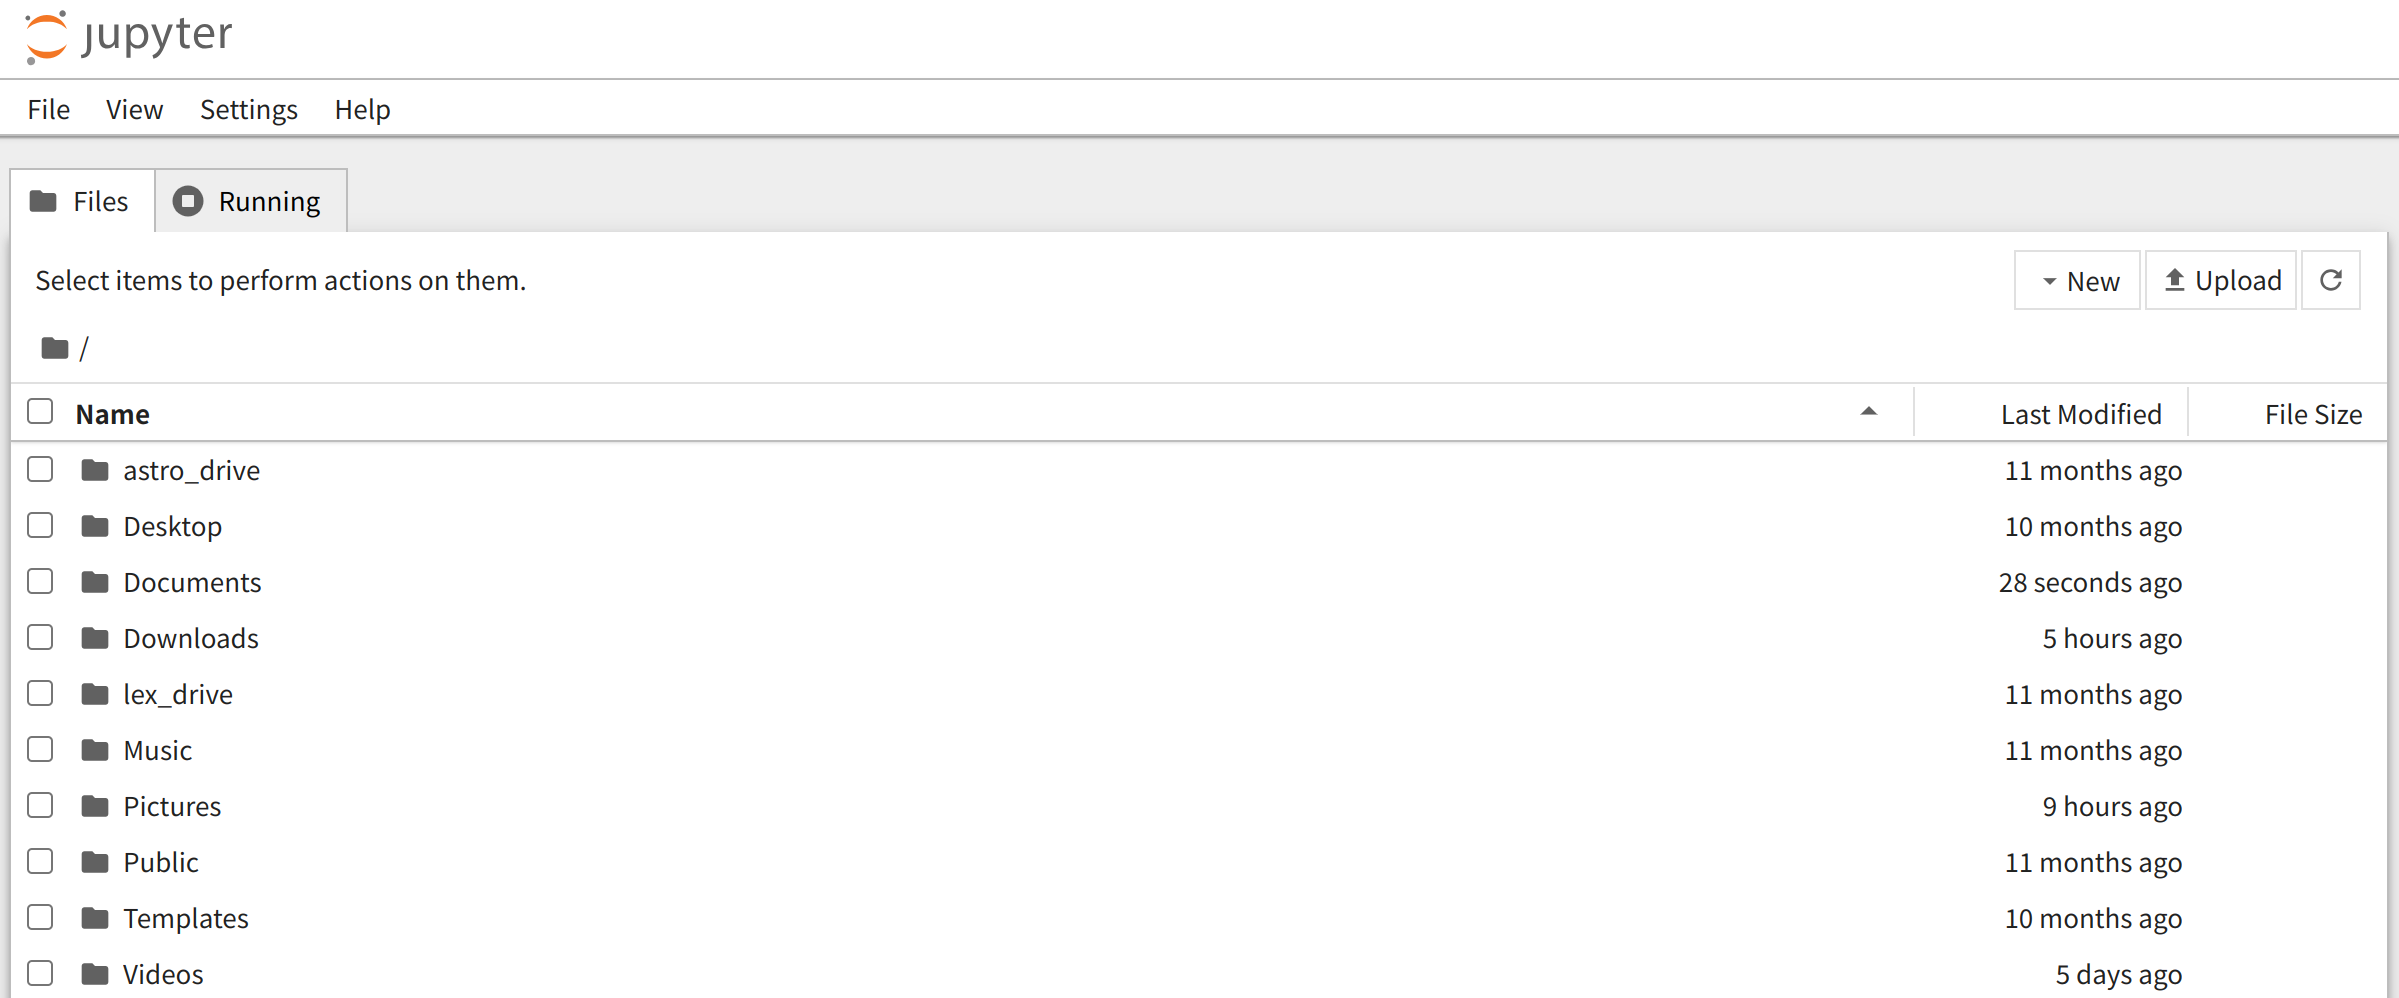
\includegraphics[width=\linewidth]{figures/jupyter-interface.png}
    \caption{Interfaz gráfica de Jupyter Notebook}
    \label{fig:jupyter-interface}
\end{figure}

Desde la interfaz de Jupyter dirígete a tu carpeta de trabajo y crea un nuevo Notebook. Para lograrlo, haz click en el botón <<\norbash{New}>> en la esquina superior derecha y selecciona la opción <<\norbash{Notebook}>>, luego elige el \emph{kernel} llamado <<\norbash{Python 3 (ipykernel)}>> y esto abrirá una nueva pestaña en tu navegador. 

\begin{figure}[htb]
    \centering
    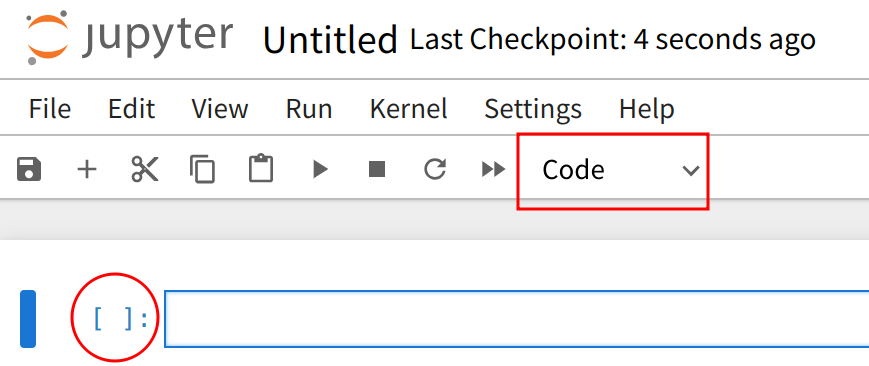
\includegraphics[width=0.48\linewidth]{figures/Jupyter-code.png} \hfill 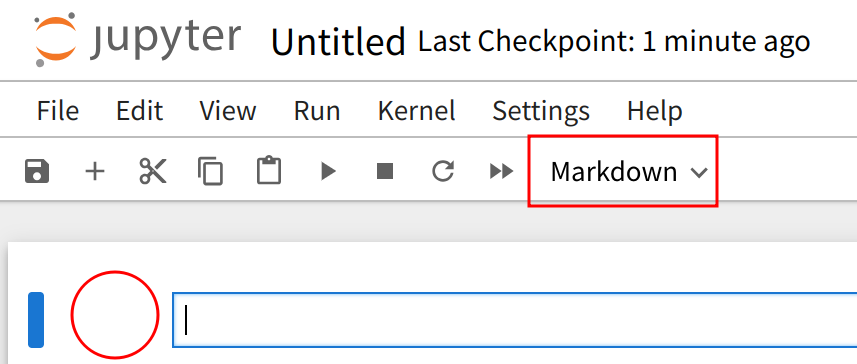
\includegraphics[width=0.48\linewidth]{figures/jupyter-markdown.png}
    \caption{Opciones disponibles para escribir en Jupyter}
    \label{fig:jupyter-code-markdown}
\end{figure}

En esa nueva pestaña, verás que aparecen los caracteres \pynorm{[]:} (encerrado con un círculo rojo en el panel izquierdo de la Figura \ref{fig:jupyter-code-markdown}) y a la derecha aparece una celda vacía donde puedes escribir los comandos de Python. Los caracteres \pynorm{[]:} en Jupyter Notebook son el equivalente a los caracteres \pynorm{>>>} en la terminal. 

En la parte superior del Notebook hay una barra de menú, que a su vez contiene un botón con la palabra <<\norbash{Code}>> (encerrada con un rectángulo rojo en el panel izquierdo de la Figura \ref{fig:jupyter-code-markdown}). Al darle clic se muestra un menú desplegable cuyas opciones son <<\norbash{Code}>> y <<\norbash{Markdown}>>. Este último es un tipo de \emph{lenguaje de marcas} bastante popular para escribir texto con formato. Si seleccionas <<\norbash{Markdown}>>, los símbolos \pynorm{[]:} de la celda desaparecen (como se muestra en el panel derecho de la Figura \ref{fig:jupyter-code-markdown}) y ahora puedes escribir texto, ecuaciones, imágenes y más. Puedes revisar algunas nociones básicas sobre la escritura de texto Markdown en este enlace de \href{https://docs.github.com/en/get-started/writing-on-github/getting-started-with-writing-and-formatting-on-github/basic-writing-and-formatting-syntax}{Github Docs}. 

Cuando vas a escribir código, siempre debes verificar que la celda está en modo <<\norbash{Code}>> o en su defecto, que a la izquierda de la celda aparezcan los símbolos \pynorm{[]:}, de lo contrario, tus comandos no se ejecutarán. Por ejemplo, da clic en la celda vacía y asegúrate que se encuentre en modo <<\norbash{Code}>> y escribe el comando \pynorm{print("¡Hola mundo!")}. Para ejecutar el código de una celda, debes dar click a la celda y usar la combinación de teclas \bashbold{Shift+Enter}. El resultado debería ser algo similar a lo siguiente:

\begin{pyin}
print("¡Hola mundo!")
\end{pyin}
\begin{pyprint}
¡Hola mundo!
\end{pyprint}

Para cerrar correctamente Jupyter Notebook, dirige tu cursor hacia la esquina superior izquierda del Notebook y selecciona \norbash{File -> Shutdown}. Una vez que lo hagas, podrás cerrar esa pestaña del navegador. Debes repetir este procedimiento para todas las pestañas del Notebook abiertas. Como último dato sobre Jupyter Notebook, debes saber que aunque necesite de un navegador web para funcionar, en realidad no necesita de una conexión a internet para ejecutar los comandos. El navegador web es únicamente para la interfaz gráfica.

\subsubsection{Visual Studio Code y PyCharm}
Visual Studio Code (VS Code) y PyCharm son otros IDEs muy populares que también trabajan con Notebooks de Python y también archivos de texto plano con extensión \texttt{.py}. Su interfaz es similar a la de Jupyter Notebook y funcionan de la misma manera. Puedes revisar las instrucciones de instalación y configuración de VS Code y PyCharm en los sitios web oficiales \url{https://code.visualstudio.com/} y \url{https://www.jetbrains.com/es-es/pycharm/download/}, respectivamente. 

Como última opción, si no te es posible instalar Python en tu computadora, puedes utilizar la opción en línea llamada Google Colaboratory (o simplemente Colab), a la que puedes acceder desde tu cuenta de google drive. La ventaja de usar Colab es que no necesitas instalar nada en tu computadora y puedes usar todos los paquetes de Python que requieras. Sin embargo, sí necesitarás de una conexión a internet para poder utilizarlo.

PyCharm, VS Code, Colab y Jupyter Notebook son totalmente equivalentes entre sí, teniendo diferencias mínimas y por lo tanto puedes utilizar el IDE que sea de tu preferencia. Teniendo esto en cuenta, podemos iniciar con algunas nociones sobre la escritura de código Python usando Notebooks.

\subsection{Python como calculadora}
\subsubsection{Operaciones aritméticas}
Una de las formas elementales en las que Python puede ser utilizado es como una calculadora. En este sentido, la Tabla \ref{tab:aritmetic-operators} muestra las operaciones aritméticas que pueden ejecutarse con Python. Quizá no estés muy familiarizado con las operaciones de división entera (representada con los caracteres \pynorm{//}) y división modular (representada con el carácter \mintinline[style=friendly]{python}{%}), pero las revisaremos con detalle más adelante.

\begin{table}[htb]
    \centering
    \caption{Operadores aritméticos}
    \label{tab:aritmetic-operators}
    \begin{tabular}{c|c} \hline
        Símbolo/Operador & Significado/Operación \\ \hline
        + & Suma \\
        - & Resta \\
        * & Multiplicación \\
        / & División \\
        ** & Exponenciación \\
        // & División entera \\
        \% & División modular \\ \hline
    \end{tabular} 
\end{table}

Abre una nueva terminal de comandos, activa tu entorno virtual de Python e inicia una nueva sesión de Jupyter Notebook. Puedes abrir el mismo Notebook que creaste anteriormente o crear uno nuevo. Asegúrate que las celdas estén en modo <<\norbash{Code}>> e intenta ejecutar los siguientes comandos. El resultado de cada comando se mostrará al lado de los caracteres {\color{myorange}\pynorm{[]:}} (en color naranja). 

Veamos cómo funcionan los operadores aritméticos con unos ejemplos sencillos. Comenzamos con una simple, para calcular el valor de la operación $5+9$:

\begin{pyin}
5 + 9
\end{pyin}
\begin{pyout}
14
\end{pyout}

La siguiente expresión es equivalente a $40 - 5\times 4$:
\begin{pyin}
40 - 5*4
\end{pyin}
\begin{pyout}
20
\end{pyout}

Y también podemos agrupar términos utilizando los paréntesis. Por ejemplo, podemos calcular el valor de la expresión $(40 - 5\times 4)/4$ usando la siguiente sintaxis:
\begin{pyin}
(40 - 5 * 4) / 4
\end{pyin}
\begin{pyout}
5.0
\end{pyout}

Y para calcular el valor de $3^2 + 4^2$ se usa la sintaxis:
\begin{pyin}
4**2 + 3**2
\end{pyin}
\begin{pyout}
25
\end{pyout}

Ahora revisemos con un poco de detalle el operador \pynorm{//}, que en Python es el operador de división entera. Este operador divide dos números y redondea el resultado hacia abajo al número entero más cercano. Por ejemplo, sabemos que $7/3 = 2.333$. Si aplicamos el operador de división entera a esos mismos números se obtiene:
\begin{pyin}
7 // 3
\end{pyin}
\begin{pyout}
2
\end{pyout}

En este caso, \pynorm{7 // 3} es igual a $2$ porque la parte fraccionaria ($0.333...$) se descarta. Ahora veamos cómo se comporta este operador con números negativos:
\begin{pyin}
-7 // 3
\end{pyin}
\begin{pyout}
-3
\end{pyout}

En este caso, \pynorm{-7 // 3} es igual a \pynorm{-3} porque el resultado se redondea hacia abajo (es decir, al entero más negativo).

Por otro lado, el operador \% en Python es el operador de división modular (también conocido como resto o residuo). Este operador devuelve el resto de la división entre dos números. Es útil para determinar si un número es divisible por otro, o para obtener la parte sobrante después de dividir un número por otro. Veamos cómo funciona con ejemplos:
\begin{pyin}
7 % 3
\end{pyin}
\begin{pyout}
1
\end{pyout}
En este caso, \mintinline[style=friendly]{python}{7 % 3} es igual a $1$ porque $7$ dividido entre $3$ es igual a $2$ con un residuo de $1$.

\subsubsection{Operaciones matemáticas avanzadas}
Para realizar operaciones matemáticas más avanzadas, necesitaremos utilizar un \emph{módulo} de Pytho llamado \pynorm{math}. Un módulo es un archivo que contiene definiciones y declaraciones de Python, como funciones, variables y clases. Los módulos permiten organizar y reutilizar código.

Para usar el módulo \pynorm{math}, debemos importarlo en nuestro código. La forma más sencilla de hacerlo es usando la palabra clave <<\pynorm{import}>>. Dentro del módulo \pynorm{math} están definidas muchas funciones matemáticas como la raíz cuadrada, logaritmos, funciones trigonométricas y mucho más. Para usarlas, debemos hacerlo con el operador de acceso, que en Python es un punto. La siguiente celda de código muestra cómo importar el módulo \pynorm{math} y cómo acceder a la función raíz cuadrada, definida como \pynorm{sqrt} dentro de dicho módulo:

\begin{pyin}
import math

print(math.sqrt(16))
\end{pyin}
\begin{pyprint}
4.0
\end{pyprint}

También podemos hacer importaciones específicas de las funciones dentro del módulo. Para esto usamos la palabra <<\pynorm{from}>>. El siguiente ejemplo muestra cómo importar la función \pynorm{sqrt} definida dentro del módulo \pynorm{math}:
\begin{pyin}
from math import sqrt

print(sqrt(16))
\end{pyin}
\begin{pyprint}
4.0
\end{pyprint}
En este último caso, no fue necesario escribir \pynorm{math.sqrt} para calcular la raíz cuadrada, porque importamos directamente la función \pynorm{sqrt}. 

Adicionalmente, puedes importar módulos o funciones específicas y renombrarlas a tu gusto usando la palabra <<\pynorm{as}>>. Los siguientes dos ejemplos muestran cómo funciona esta sintaxis.

\begin{pyin}
import math as m

print(m.sqrt(16))
\end{pyin}
\begin{pyprint}
4.0
\end{pyprint}

\begin{pyin}
from math import sqrt as raiz_cuadrada

print(raiz_cuadrada(16))
\end{pyin}
\begin{pyprint}
4.0
\end{pyprint}

Como normal general, se recomienda hacer todas las importaciones al inicio del programa y utilizar alias claros y fácilmente identificables. 

\chapter{Variables y contenedores}
%\counterwithout{section}{chapter}

% Setting the cell notebooks again to zero
\setcounter{ipythcntr}{0}

%Introduction
\section{Introducción}
En cualquier lenguaje de programación, las variables actúan como nombres simbólicos que almacenan datos, permitiéndonos utilizar la información de manera eficiente a lo largo de nuestros programas. Los contenedores, por otro lado, son estructuras de datos que permiten agrupar múltiples valores en una sola entidad, facilitando la organización y gestión de conjuntos de datos. A lo largo de esta lección, aprenderemos cómo declarar variables, entenderemos los tipos de datos básicos y profundizaremos en los contenedores más utilizados en Python, como listas, tuplas, conjuntos y diccionarios.

\subsection{Variables}

Las variables son parte fundamental en cualquier lenguaje de programación y constan simplemente de dos partes: el nombre de la variable y su valor. Ambas partes están separadas por el signo de igual (\pynorm{=}). Es decir, se escribe el nombre de la variable a la izquierda del símbolo \pynorm{=} y su valor se escribe a la derecha. Si se quisiera por ejemplo definir una variable llamada \pynorm{var_1} y asignarle el valor numérico \(53\), se haría de la siguiente manera:

\begin{pyin}
var_1 = 53
\end{pyin}

Los nombres de las variables pueden contener letras minúsculas, mayúsculas, dígitos (\pynorm{0 - 9}) y guiones bajos (\pynorm{_}). Sin embargo, los nombres no pueden empezar con dígitos; deben iniciar necesariamente con una letra o un guion bajo. Por ejemplo, los nombres <<\pynorm{_var}>>, <<\pynorm{_var1}>> o <<\pynorm{_var_1}>> son válidos, pero <<\pynorm{1_var}>> y <<\pynorm{1var}>> son nombres no permitidos y devuelven un error, como puedes verificar con el siguiente ejemplo:

\begin{pyin}
1var = 53
\end{pyin}

\begin{pyerror}
    Cell In[1], line 1
    1var = 53
    ^
SyntaxError: invalid decimal literal    
\end{pyerror}

El mensaje de error nos indica que estamos colcando un valor numérico en una posición inválida al momento de definir la variable.

\subsubsection{Variables tipo int/float}

En Python se distinguen dos tipos principales de variables numéricas: las variables tipo \pybold{int}, que corresponden a los números enteros y las variables tipo \pybold{float}, que corresponden a números decimales o muy grandes escritos con notación científica. Por ejemplo, la variable definida anteriormente y que llamamos \pynorm{var_1} es de tipo \pybold{int}. En cambio, los valores numéricos \(1.5\) y \(4 \times 10^{3}\) son de tipo \pybold{float}. En realidad, la diferencia entre variables tipo \pybold{int} y \pybold{float} es más complicada que simplemente eso, pero no entraremos en detalles. En el siguiente ejemplo se definen dos variables tipo \pybold{float}.

\begin{pyin}
var_2 = 1.5
var_3 = 4e3
\end{pyin}

Nota cómo la expresión \(4 \times 10^{3}\) se sustituye por \pynorm{4e3}, haciendo muy fácil escribir expresiones con valores numéricos grandes. Las variables \pybold{int} y \pybold{float} admiten las operaciones aritméticas vistas en la Clase 1. Al realizar una operación aritmética entre un \pybold{int} y un \pybold{float}, el resultado será un \pybold{float}.

\subsubsection{Variables de tipo string}
Otro tipo de variables son las de tipo \emph{string} (o cadena de caracteres), que se caracterizan porque son un conjunto de palabras o caracteres formando un mensaje, tales como <<¡Hola mundo!>>. En Python, estas variables se identifican como de tipo \pybold{str} y para definirlas se debe escribir el mensaje que queramos dentro de comillas simples (\pynorm{'}) o comillas dobles (\pynorm{"}). Esto se muestra en el siguiente ejemplo:

\begin{pyin}
message_1 = 'Hola'
message_2 = "y buenos días" 
\end{pyin}

Es posible aplicar las operaciones aritméticas de suma y multiplicación a las variables \pybold{str}. Al aplicar la suma a las variables \pynorm{message_1} y \pynorm{message_2} se forma una nueva oración. Intenta ejecutar las siguientes dos celdas de código:

\begin{pyin}
message_4 = message_1 + message_2
print(message_4)
\end{pyin}

\begin{pyprint}
Holay buenos días
\end{pyprint}

\begin{pyin}
message_5 = message_1 + ' ' + message_2
print(message_5)
\end{pyin}
    
\begin{pyprint}
Hola y buenos días
\end{pyprint}

La diferencia entre las variables \pynorm{message_4} y \pynorm{message_5} es que a \pynorm{message_5} se le agregó explícitamente un espacio en blanco (\pynorm{' '}) al momento de sumar las variables \pynorm{message_1} y \pynorm{message_2}. Las variables \pybold{str} no pueden sumarse con variables tipo \pybold{int} ni \pybold{float}.


Por otro lado, la multiplicación de una variable \pybold{str} y una de tipo \pybold{int} sí está permitida. Intenta ejecutar lo siguiente:

\begin{pyin}
message_1 * 3
\end{pyin}

\begin{pyout}
HolaHolaHola
\end{pyout}

En resumen, se multiplicó \pynorm{message_1} por el número \pynorm{3}, y el mensaje apareción tres veces. Las variables \pybold{str} no pueden ser multiplicadas por variables tipo \pybold{float}


\subsubsection{Comentarios}

Los comentarios son parte esencial de cualquier lenguaje de programación. Se trata de líneas de código que son ignorados por el intérprete/compilador y sirven para documentar el código. Mientras más líneas de código escribas, más difícil será recordar qué hace cada línea o bloque de código. Debido a esto se hacen necesarios los comentarios, y en Python hay dos formas de escribirlos. La primera es usando el símbolo de numeral: \mintinline[style=friendly]{python}{#}. Cualquier cosa que escribamos después del símbolo será ignorada por Python:

\begin{pyin}
pi = 3.14159265     #- Una variable float

num = 5             #- Una variable int
    
message = "nueve"   #- Una variable str
\end{pyin} 

En la primera línea del ejemplo anterior, se declaró una variable llamada \pynorm{pi} y se le asignó un valor de \pynorm{3.14159265} y seguidamente se escribió un comentario para aclarar el tipo de variable que se está definiendo. Esto se repitió para las variables \pynorm{num} y \pynorm{message}. 

La otra forma de escribir comentarios consisten en colocarlos dentro de triples comillas simples (\pynorm{''' '''}) o triples comillas dobles (\pynorm{""" """}). Las triples comillas permiten que el texto entre ellas abarque más de una sola línea. En realidad, estas son un tipo especial de comentarios que se utilizan para documentar las funciones, métodos, clases o módulos y por lo tanto son llamadas \emph{docstrings} (cadenas de documentación). 

\subsubsection{Variables tipo bool}
Las variables tipo bool, o variables booleanas son aquellas que solo pueden tomar dos posibles valores: \pybold{True} (verdadero) o \pybold{False} (falso), a las cuales corresponden los valores numéricos de \pynorm{0} y \pynorm{1}, respectivamente. Este tipo de variables aparecen cuando se hacen comparaciones entre una o más variables. Para eso se utilizan operadores de comparación, de los cuales, los más comunes se muestran en la Tabla \ref{tab:comparison-operators}

\begin{table}[htb]
    \centering
    \caption{Operadores de comparación}
    \label{tab:comparison-operators}

    \begin{tabular}{c c} \hline
        Operador & Significado \\ \hline
        \pynorm{>} & Mayor que \\
        \pynorm{<} & Menor que \\
        \pynorm{>=} & Mayor o igual que \\
        \pynorm{<=} & Menor o igual que \\
        \pynorm{==} & Igual que \\
        \pynorm{!=} & Diferente de \\ \hline        
    \end{tabular}
\end{table}

Por ejemplo, sabemos que el número \pynorm{3} es menor que el número 5. Entonces la expresión \pynorm{3 > 5} es falsa, como puedes comprobarlo:

\begin{pyin}
3 > 5
\end{pyin}
\begin{pyout}
False
\end{pyout}

Estos operadores también pueden ser acompañados por las palabras clave definidas en Python: \pybold{and} y \pybold{or}. Intenta ejecutar los siguientes ejemplos:

\begin{pyin}
5 <= 2 and 4 > 2
\end{pyin}
\begin{pyout}
False
\end{pyout}

Veamos con detalle qué es lo que está pasando en este ejemplo. El número \pynorm{5} es mayor que \pynorm{2}, por lo tanto, la expresión \pynorm{5 <= 2} es falsa. Por otro lado, el número \pynorm{4} es mayor que \pynorm{2}, por lo tanto, la expresión \pynorm{4 > 2} es verdadera. En otras palabras, la expresión es quivalente a: \pynorm{False and True}. El operador \pybold{and} devuelve un valor verdadero únicamente si todas las expresiones son verdaderas, de lo contrario devuelve un valor falso. Ya que en este caso una de las expresiones es falsa, entonces el resultado es \pybold{False}. Ahora revisa el siguiente ejemplo:

\begin{pyin}
5 <= 2 or 4 > 2
\end{pyin}
\begin{pyout}
True
\end{pyout}

Estamos haciendo las mismas comparaciones que en el ejemplo anterior, pero ahora con el operador \pybold{or}, el cual devuelve un valor falso únicamente si todas las expresiones son falsas, de lo contrario devuelve un valor verdadero. En este caso, la expresión de la derecha es verdadera y por lo tanto, el resultado es un valor \pybold{True}.

Las variables booleanas se utilizan para iniciar, terminar o repetir algún proceso dependiendo si alguna condición se cumple o no. Esto lo veremos más adelante cuando trabajemos con controladores de flujo.

\subsection{Contenedores}
Los contenedores son un tipo de estructuras de datos que se utilizan para almacenar múltiples elementos o variables bajo un solo nombre. A diferencia de las variables, que pueden contener un único valor a la vez, los contenedores permiten mantener una colección de valores, los cuales a su vez pueden ser otros contenedores. Los contenedores son fundamentales para manejar datos de manera eficiente en Python, ya que permiten agrupar, iterar, acceder y manipular conjuntos de valores de manera ordenada y flexible. Los contenedores disponibles en python son las listas, tuplas, conjuntos y diccionarios.

\subsubsection{Listas}
Las listas son secuencias ordenadas de elementos o variables de cualquier tipo, que no tienen que estar relacionadas entre sí. Para definir una lista se se colocan los elementos separados por comas y encerrados entre corchetes. El siguiente ejemplo muestra que una lista puede contener cualquier tipo de variable:

\begin{pyin}
lista_1 = [1, 'Uno', True]
print(lista_1)
\end{pyin}
\begin{pyprint}
[1, 'Uno', True]
\end{pyprint}

También es posible que una lista contenga a otras listas:
\begin{pyin}
lista_2 = [lista_1, [0, 'Cero', False]]
\end{pyin}
\begin{pyprint}
[[1, 'Uno', True], [0, 'Cero', False]]
\end{pyprint}

Además, el operador numérico de la suma está permitido en las listas. El resultado es una nueva lista:
\begin{pyin}
lista_3 = lista_1 + lista_2
print(lista_3)
\end{pyin}
\begin{pyprint}
[1, 'Uno', True, [1, 'Uno', True], [0, 'Cero', False]]
\end{pyprint}

Como se mencionó, las listas son una colección ordenada de elementos. Debido a esta característica, sus elementos pueden ser accedidos mediante índices, que corresponden a la posición del elemento en la lista. Sin embargo, se debe tener en cuenta que Python es un lenguaje de programación que comienza a contar desde el número cero. Es decir, al primer elemento le corresponde la posición (o índice) \pynorm{0}, al segundo elemento la posición \pynorm{1} y así sucesivamente. Por ejemplo, definamos una nueva lista con los nombres de algunos astrónomos:

\begin{pyin}
astronomers = ['Carl Sagan', 'Stephen Hawking', 'Jocelyn Bell']
\end{pyin}

Para acceder a un elemento de la lista \pynorm{astronomers}, se escribe el nombre de la lista y se acompaña del índice encerrado entre corchetes y sin espacios. Específicamente, para acceder a \pynorm{'Carl Sagan'}, que es el primer elemento, lo hacemos de la siguiente manera:

\begin{pyin}
astronomers[0] # Selecciona el primer elemento
\end{pyin}
\begin{pyout}
'Carl Sagan'
\end{pyout}

El último elemento de cualquier lista, independiente de cuántos elementos tenga, puede ser accedido mediante el índice \pynorm{-1}, como puedes verificar:

\begin{pyin}
astronomers[-1] # Selecciona el último elemento
\end{pyin}
\begin{pyout}
'Jocelyn Bell'
\end{pyout}

Una de las características de las listas es que sus elementos pueden ser modificados. En un contexto de programación, esto significa que las listas son \emph{mutables}. Por ejemplo, para reemplazar el primer elemento de la lista por el nombre algún otro astrónomo, podemos hacerlo de la siguiente manera:

\begin{pyin}
astronomers[0] = 'Johannes Kepler'
print(astronomers)
\end{pyin}
\begin{pyprint}
['Johannes Kepler', 'Stephen Hawking', 'Jocelyn Bell']
\end{pyprint}

Puedes agregar elementos a una lista usando el método \pynorm{list.append()} (el cual permite agregar un elemento a la vez) y el método \pynorm{list.extend()} (el cual permite agregar varios elementos a la vez, en formato de lista). Ambos métodos agregan los elementos al final de la lista. Por ejemplo, para agregar nuevamente a Carl Sagan a la lista de astrónomos, podemos hacerlo de la siguiente manera: 

\begin{pyin}
astronomers.append('Carl Sagan')
print(astronomers)
\end{pyin}
\begin{pyprint}
['Johannes Kepler', 'Stephen Hawking', 'Jocelyn Bell', 'Carl Sagan']
\end{pyprint}

Podemos en cambio, agregar dos elementos al mismo tiempo de la siguiente manera:

\begin{pyin}
astronomers.extend(['Henrietta Leavitt', 'Vera Rubin'])
print(astronomers)
\end{pyin}
\begin{pyprint}
['Johannes Kepler', 'Stephen Hawking', 'Jocelyn Bell', 'Carl Sagan', 'Henrietta Leavitt', 'Vera Rubin']
\end{pyprint}

Algunos tipos de variables permiten ser convertidos a listas, como es el caso de las variables de tipo \pybold{str}. Para lograrlo, se utiliza la función \pynorm{list()} predefinida en Python. Revisa el siguiente ejemplo:

\begin{pyin}
letters = list(astronomers[2])
print(letters)
\end{pyin}
\begin{pyprint}
['J', 'o', 'c', 'e', 'l', 'y', 'n', ' ', 'B', 'e', 'l', 'l']
\end{pyprint}

Adicionalmente, las variables de tipo \pybold{str} también admiten acceder a sus elementos mediante índices:

\begin{pyin}
name = 'Jocelyn'
name[0]
\end{pyin}
\begin{pyout}
'J'
\end{pyout}

También puedes definir listas que sean una porción de otra lista. A esto se le conoce como <<\emph{rebanar}>> o en inglés, <<\emph{slice}>>. Supongamos por ejemplo, que solo queremos seleccionar los primeros 3 elementos de la lista \pynorm{astronomers}, entonces usamos la siguiente sintaxis:

\begin{pyin}
new_astronomers = astronomers[0:3]
print(new_astronomers)
\end{pyin}
\begin{pyprint}
['Johannes Kepler', 'Stephen Hawking', 'Jocelyn Bell']
\end{pyprint}

El ejemplo anterior está seleccionando los elementos de la lista que van desde el índice \pynorm{0} (primer elemento) hasta el índice {3} (cuarto elemento). Por defecto en Python, el índice despúes de los dos puntos (\pynorm{:}) no se incluye, por eso la lista \pynorm{new_astronomers} solo tiene tres elementos y no cuatro.

\subsubsection{Tuplas}
Las tuplas representan la versión inmutable de las listas, es decir, pueden almacenar cualquier tipo de elementos pero sus valores no se pueden modificar. Para definirlas, basta con escribir los elementos separados por comas sin encerrarlos:

\begin{pyin}
planets_1 = 'Mercurio', 'Venus', 'Tierra'
planets_1
\end{pyin}
\begin{pyout}
('Mercurio', 'Venus', 'Tierra')
\end{pyout}

Alternativamente, las tuplas se definen al escribir los elementos separados por comas y encerrarlos entre paréntesis:

\begin{pyin}
planets_2 = ('Marte', 'Júpiter', 'Saturno')
planets_2
\end{pyin}
\begin{pyout}
('Marte', 'Júpiter', 'Saturno')
\end{pyout}

Al igual que en el caso de las listas, se puede acceder a los elementos de una tupla mediante índices y se puede convertir una variable de tipo \pybold{str} a una tupla usando la función \pynorm{tuple()}. usando esa misma función, también puedes convertir una lista en una tupla.

\subsubsection{Conjuntos}
Los conjuntos (en inglés llamados <<\emph{sets}>>) son colecciones de datos no ordenados y además no permiten elementos duplicados. Esto significa que no es posible acceder a sus elementos mediante índices y que ninguno de sus elementos se repite. Los conjuntos se definen con sus elementos separados por comas y encerrados entre llaves:

\begin{pyin}
my_set = {1,2,3,4,5,5,5}
print(my_set)
\end{pyin}
\begin{pyprint}
{1, 2, 3, 4, 5}
\end{pyprint}

También puedes definirlos con la función \pynorm{set()}:
\begin{pyin}
my_set = set([1,2,3,4,5,5,5])
\end{pyin}
\begin{pyprint}
{1, 2, 3, 4, 5}
\end{pyprint}

Los conjuntos también son contenedores mutables. Para añadir elementos se utiliza la función \pynorm{add()}:
\begin{pyin}
my_set.add(6)
print(my_set)
\end{pyin}
\begin{pyprint}
{1, 2, 3, 4, 5, 6}
\end{pyprint}

Para eliminar un elemento se utilizan los métodos \pynorm{remove()} o \pynorm{doscard()}, como puedes comprobar:

\begin{pyin}
my_set.remove(3) 
print(my_set) 
\end{pyin}
\begin{pyprint}
{1, 2, 4, 5, 6}
\end{pyprint}

\begin{pyin}
my_set.discard(2)
print(my_set) 
\end{pyin}
\begin{pyprint}
{1, 4, 5, 6}
\end{pyprint}
La diferencia en ambos métodos es que \pynorm{remove()} lanzará un error si el elemento no existe, mientras que \pynorm{discard()} no hará nada si el elemento no está presente.

También puedes usar el operador \pybold{in} para verificar si un elemento está en el conjunto. Ten en cuenta que este operador también puede utilizarse para verificar si un elemento está en una lista o en una tupla. Veamos un ejemplo solo para los conjuntos:

\begin{pyin}
print(2 in my_set)
\end{pyin}
\begin{pyprint}
False
\end{pyprint}

Otras operaciones disponibles para los conjuntos son:
\begin{itemize}
    \item \textbf{Unión:} combina todos los elementos de dos conjuntos, eliminando los duplicados, mediante el operador <<\pynorm{|}>>.
    \item \textbf{Intersección:} Devuelve los elementos comunes en ambos conjuntos, mediante el operador <<\pynorm{&}>>.
    \item \textbf{Diferencia:} Devuelve los elementos que están en el primer elemento pero no en el segundo, mediante el operador <<\pynorm{-}>>.
    \item \textbf{Diferencia simétrica:} Devuelve los elementos que están en un set o en otro, pero no en ambos, mediante el operador <<\pynorm{^}>>.
\end{itemize}

\subsubsection{Diccionarios}
Los diccionarios son estructuras de datos no ordenados y están compuestos de pares \emph{clave-valor} (en inglés \emph{key-values}), donde cada valor está asociado a una clave única. Para crear un diccionario se escriben los pares de clave-valor sperados por comas y encerrados con llaves \pynorm{{}}, o encerrados por la función \pynorm{dict()}. Para entenderlo mejor, revisa el siguiente ejemplo:

\begin{pyin}
stephen = {
    "first_name": "Stephen", 
    "last_name": "Hawking", 
    "birthday": (8, 1, 1942)
    }
print(stephen)
\end{pyin}
\begin{pyprint}
{'first_name': 'Stephen', 'last_name': 'Hawking', 'birthday': (8, 1, 1942)}   
\end{pyprint}
\begin{pyin}
albert = dict(
    first_name="Albert", 
    last_name='Einstein',
    birthday= (14, 3, 1879) 
    )
print(albert)
\end{pyin}
\begin{pyprint}
{'first_name': 'Albert', 'last_name': 'Einstein', 'birthday': (14, 3, 1879)}
\end{pyprint}

Las dos sintaxis anteriores son totalmente equivalentes para definir un diccionario. Para acceder a cualquier valor de un diccionario, se escribe el nombre del dicionario y en seguida, encerrado entre corchetes se escribe su clave correspondiente. Por ejemplo:

\begin{pyin}
stephen['first_name']
\end{pyin}
\begin{pyout}
'Stephen'
\end{pyout}

Los diccionarios son contendores mutables, por lo tanto sus valores pueden cambiar, pero no sus claves. Puedes agregar un par clave-valor simplemente asignando un valor a una nueva clave:

\begin{pyin}
stephen['nationality'] = "British"
print(stephen)
\end{pyin}
\begin{pyprint}
{'first_name': 'Stephen', 'last_name': 'Hawking', 'birthday': (8, 1, 1942), 'nationality': 'British'}
\end{pyprint}

Puedes obtener todas las claves, valores, o pares clave-valor usando los métodos \pynorm{keys()}, \pynorm{values()} y \pynorm{items()}, respectivamente:

\begin{pyin}
albert.keys()
\end{pyin}
\begin{pyout}
dict_keys(['first_name', 'last_name', 'birthday'])
\end{pyout}

\begin{pyin}
albert.values()
\end{pyin}
\begin{pyout}
dict_values(['Albert', 'Einstein', (14, 3, 1879)])
\end{pyout}

\begin{pyin}
albert.items()
\end{pyin}
\begin{pyout}
dict_items([('first_name', 'Albert'), ('last_name', 'Einstein'), ('birthday', (14, 3, 1879))])
\end{pyout}
\chapter{Control de flujo y lógica}

% Setting the cell notebooks again to zero
\setcounter{ipythcntr}{0}

\section{Controles de flujo}
Los controles de flujo en un lenguaje de programación permiten que ciertas partes de un código se ejecuten y otras no, dependiendo de si se cumplen o no algunas condiciones. Adicionalmente, también permiten ejecutar líneas de código una y otra vez mientras alguna condición siga siendo válida. Debido a esto, los principales controles de flujo y lógica son llamados \emph{condicionales} y \emph{bucles} (en inglés, \emph{loops}). En esta clase revisaremos ambos conceptos.

\subsection{Condicionales}
Son el tipo de controladores de flujo más sencillos, su funcionamiento puede describirse de la siguiente manera: "Si la variable $x$ es verdadera, entonces realiza una tarea; en caso contrario, realiza esta otra tarea". Para escribir este tipo de condiciones se utilizan las palabras en inglés <<if>> y <<else>>, que significan <<si>> y <<en caso contrario>>, respectivamente.  

\subsubsection{Declaraciones if}
La forma más sencilla de usar los condicionales es cuando solo se quiere comprobar si alguna condición es verdadera y no hacer nada si la condición es falsa. En ese caso, se utiliza la palabra clave \pybold{if} una única vez. La sintaxis es la siguiente:

\begin{shell}
if <condition>:
    <if-block>
\end{shell}

Para este tipo de declaraciones, la condición, identificada como \pynorm{<condition>} puede ser cualquier tipo de expresión de comparación o lógica que devuelva un valor \pybold{True} o \pybold{False}. Además, inmediatamente después de dicha condición se escriben dos puntos (\pynorm{:}). El segmento \pynorm{<if-block>} representa aquellos comandos o instrucciones que se ejecutarán únicamente si la condición es verdadera.

Algo muy importante es que los comandos del \pynorm{<if-block>} deberán ser escritos abajo del <<\pynorm{if <condition>:}>> con una sangría (en inglés <<\emph{indent}>>) de cuatro espacios. En Python, esta sangría es obligatoria siempre que se quiera separar bloques de código del resto de líneas de código. De no usar la sangría de cuatro espacios en los condicionales, el código generará un error. Como ejemplo, intenta ejecutar la siguiente celda de código:

\begin{pyin}[]
#- Definiendo un número
number = 0 
if number == 0.0:
print(f"El número {number} es igual a 0.0")
\end{pyin}
\begin{pyerror}
  Cell In[1], line 3
    print(f"El número {number} es igual a 0.0")
    ^
IndentationError: expected an indented block after 'if' statement on line 2
\end{pyerror}

Este error es bastante simple. Python nos está diciendo que se esperaba un bloque con sangría después de la declaración \pynorm{if}. Puedes corregirlo simplemente agregando la sangría de cuatro espacios:

\begin{pyin}[]
#- Definiendo un número
number = 0 
if number == 0.0:
    print(f"El número {number} es igual a 0.0")
\end{pyin}
\begin{pyout}
El número 0 es igual a 0.0
\end{pyout}

La condición \pynorm{number == 0.0} es verdadera y por lo tanto se mostró el mensaje. Si la condición hubiera sido falsa, no se habría mostrado ningún mensaje. Nota cómo se definió a la variable \pynorm{number} como de tipo \pybold{int} y en la condición se comparó con una variable de tipo \pybold{float}, de modo que la condición sería equivalente a \pynorm{0 == 0.0}. Esta condición resulta ser cierta porque el operador \pynorm{==} únicamente compara si dos valores son equivalentes.

\subsubsection{Declaraciones if-else}
Cada bloque \pynorm{if} puede ir seguido de un bloque opcional \pynorm{else}, que se ejecutará únicamente si la primera condición es falsa. El bloque \pynorm{else} no necesita de ninguna condición pero sí de los dos puntos (\pynorm{:}) y la línea siguiente también debe tener sangría de cuatro espacios. La sintaxis para este tipo de declaraciones es la siguiente:

\begin{shell}
if <condition>:
    <if-block>

else:
    <else-block>
\end{shell}

Por ejemplo, podemos escribir un código que verifique si un número es par o impar, comprobando si el número es divisible por 2. Esto se puede hacer con una declaración \pynorm{if-else} de la siguiente manera:

\begin{pyin}[]
#- Definiendo un número
number = 15 

#- Comprobando si es par o impar
if number % 2 == 0:
    result = "par"
else:
    result = "impar"
    
# Muestra un mensaje con el resultado
print(f"El número {number} es {result}.")    
\end{pyin}
\begin{pyprint}
El número 15 es impar.
\end{pyprint}

El número 15 no es divisible entre dos, por lo tanto la condición \mintinline[style=friendly]{python}|number % 2 == 0| es falsa. Como resultado el bloque \pynorm{result = "par"} no se ejecuta. En cambio, se ejecuta el bloque \pynorm{result = "impar"} y se muestra el mensaje \pynorm{"El número 15 es impar"}.

\subsubsection{Declaraciones if-elif-else}
En muchas ocasiones será necesario comprobar más de dos posibles situaciones, y para esto se utiliza la sintaxis \pynorm{if-elif-else}. La palabra \emph{elif} es una abreviación de <<\emph{else if}>> en inglés y en las declaraciones pueden haber cuantos bloques \pynorm{elif} sean necesarios. El primer bloque que devuelva un valor \pybold{True} será ejecutado, y ninguno de los restantes será comprobado ni ejecutado. La sintaxis de este tipo de declaraciones es la siguiente:

\begin{shell}
if <condition>:
    <if-block>

elif <condition1>:
    <elif-block1>

elif <condition2>:
    <elif-block2>

else:
    <else-block>
\end{shell}

El siguiente ejemplo muestra cómo usar las declaraciones \pynorm{if-elif-else} para clasificar a una partícula fundamental de acuerdo a su masa:

\begin{pyin}[]
#- Masa de la partícula hipotética
mass = 5.0  # en GeV/c^2

#- Clasificación basada en su masa
if mass < 0.1:
    classification = "Mesón Ligero"

elif 0.1 <= mass < 1.0:
    classification = "Mesón Pesado"

elif 1.0 <= mass < 10.0:
    classification = "Barión"

else:
    classification = "Partícula Exótica"

#- Mostrar su classificación
print(f"La partícula con masa {mass} GeV/c^2 es un {classification}.")
\end{pyin}
\begin{pyout}
La partícula con masa 5.0 GeV/c^2 es un Barión.
\end{pyout}

Nuevamente, ten en cuenta que en cada bloque \pynorm{if-elif-else} se neesita colocar una sangría obligatoria. 

\subsubsection{Expresiones if-else}
Para finalizar con los condicionales, es posible aplicar la sintaxis \pynorm{if-else} en una simple expresión de una línea (sin los bloques de sangría). Se necesita de tres elementos y por lo tanto se le conoce como un operador condicional ternario. La sintaxis es la siguiente:

\begin{shell}
x if <condition> else y
\end{shell}

Si la condición es verdadera, entonces el resultado de la expresión anterior es \pynorm{x}, si es falsa, el resultado es \pynorm{y}. Esta expresión resulta muy útil para asignar valores a una variable con base en alguna condición. Esto se verifica en el siguiente ejemplo.

\begin{pyin}[]
#-Definiendo un número
number = -5 

#- Comprobar si es positivo o negativo y guardar el resultado
result = "positivo" if number > 0 else "negativo"

#- Mostrar el resultado
print(f"El número {number} es {result}.")
\end{pyin}
\begin{pyout}
El número -5 es negativo.
\end{pyout}

En este ejemplo, el operador ternario verifica si la variable \pynorm{number} es mayor que cero. Si de hecho lo es, le asigna el valor \pynorm{"positivo"} a la variable \pynorm{result}, en caso contrario le asigna el valor \pynorm{"negativo"}. 

\subsection{Bucles}
Como se ha visto, los condicionales permiten que los bloques de código con sangría se ejecuten una única vez dependiendo de alguna condición. Los bucles, en cambio, permiten que el mismo bloque se ejecute muchas veces. Los tipos de bucles disponibles en Python son el bucle \pynorm{while}, el bucle \pynorm{for} y algo que es conocido como <<contenedores por comprensión>>. 

\subsubsection{Bucle while}
Los bucles \pynorm{while} se relacionan con los condicionales porque permiten que el bloque de código se siga ejecutando mientras alguna condición sea verdadera. Su sintaxis es muy similar a la de las declaraciones \pynorm{if}:

\begin{shell}
while <condition>:
    <while-block>
\end{shell}

Para este tipo de declaraciones también se deben aplicar los dos puntos luego de la condición y el bloque de instrucciones también debe tener sangría. La condición es evaluada al inicio de cada iteración y si es verdadera, el bloque se ejecuta. Si la condición es falsa, el bloque es ignorado y el programa continúa. 

El ejemplo más simple usando un bucle while consiste en generar una cuenta regresiva comenzando en un número entero arbitrario:

\begin{pyin}[]
#- Número inicial
count = 5

#- Cuenta regresiva
while count > 0:
    print(count)
    count -= 1

print("¡Fin!")  # Se muestra cuando el bucle termina
\end{pyin}
\begin{pyprint}
5
4
3
2
1
¡Fin!
\end{pyprint}

En este ejemplo particular, sucede lo siguiente:
\begin{itemize}
    \item Se inicia con la variable \pynorm{count} igual a 5
    \item El bucle while se ejecuta siempre y cuando \pynorm{count} sea mayor que cero
    \item En cada iteración se imprime el valor actual de \pynorm{count} y posteriormente su valor disminuye en una unidad
    \item Eventualmente, la variable \pynorm{count} toma el valor de \pynorm{0} y la condición se vuelve falsa
    \item Cuando el bucle termina, se imprime el mensaje \pynorm{"¡Fin!"}
\end{itemize}

Es muy común cometer errores en los bucles \pynorm{while}, el más frecuente es iniciar por accidente un bucle infinito. Esto sucede cuando la condición evaluada es siempre verdadera. Si en el ejemplo anterior no hubiésemos escrito la instrucción \pynorm{count -= 1}, la variable \pynorm{count} hubiera tenido siempre un valor igual a \pynorm{5} y por lo tanto el bucle nunca habría finalizado. Al iniciar un bucle \pynorm{while} debemos asegurarnos de agregar una línea de código que haga que la condición sea falsa en algún momento. Si por algún motivo inicias un bucle infinito, siempre puedes detenerlo con la combinación de teclas \bashbold{Ctrl+C}.

También es posible terminar con el bucle \pynorm{while} en cualquier momento, haciendo uso de la instrucción \pynorm{break}. Por ejemplo, si quisiéramos encontrar el primer número par de una lista, podríamos hacerlo con el bucle \pynorm{while} de la siguiente manera:

\begin{pyin}[]
#- Lista de números
numbers = [3, 7, 12, 5, 8, 10, 15]

#- Variable para guardar el número par
first_even = None

#- Bucle while 
index = 0
while index < len(numbers):
    if numbers[index] % 2 == 0:
        first_even = numbers[index]
        break  # El bucle termina al encontrar el primer número par
    index += 1

#- Imprime el valor encontrado
if first_even is not None:
    print(f"El primer número par encontrado fue {first_even}.")
else:
    print("No hay números pares en la lista.")
\end{pyin}
\begin{pyout}
El primer número par encontrado fue 12.
\end{pyout}

\subsubsection{Bucle for}
Aunque los bucles \pynorm{while} son bastante útiles para repetir declaraciones, en general resulta de mayor utilidad el iterar sobre un contenedor (como las listas, tuplas, conjuntos y diccionarios) o algún otro tipo de variable iterable (como las cadenas de caracteres). En estos casos, se toma un elemento del contenedor en cada iteración y el bucle termina cuando ya no hay más elementos. Esto se logra usando un bucle \pynorm{for}. La sintaxis para los bucles \pynorm{for} es diferente a la del bucle \pynorm{while}, ya que no depende de ninguna condición y consta de lo siguiente:

\begin{shell}
for <variable> in <iterable>:
    <for-block>
\end{shell}

De nuevo, necesitamos escribir los dos puntos para especificar cuándo inicia el bloque de código que se va a repetir, que a su vez debe tener sangría. En la sintaxis anterior, \pynorm{<variable>} es el nombre de una variable que se asigna a un elemento cada vez que se ejecuta el bucle. El \pynorm{<iterable>} es cualquier objeto que pueda devolver elementos. Todos los tipos de contenedores vistos en la Clase 2 son iterables. La cuenta regresiva puede reescribirse de la siguiente manera usando el bucle \pynorm{for}:

\begin{pyin}
for count in [5,4,3,2,1]:
    print(count)
    
print("¡Fin!")
\end{pyin}
\begin{pyprint}
5
4
3
2
1
¡Fin!
\end{pyprint}

La instrucción \pynorm{break} también se puede usar con los bucles \pynorm{for}, y funcionan de la misma manera. Adicionalmente, también es posible utilizar la instrucción \pynorm{continue}, que ignora el bloque de código únicamente en la iteración actual y luego continua con la siguiente. Por ejemplo, el siguiente ejemplo muestra cómo ignorar los números impares en una lista:

\begin{pyin}
for num in [1, 2, 3, 4, 5, 6, 7, 8, 9]:
    if num % 2 != 0:
        continue  # Ignorar y continuar con la siguiente iteración
    print(num)

print("¡Listo!")
\end{pyin}
\begin{pyprint}
2
4
6
8
¡Listo!
\end{pyprint}

La instrucción \pynorm{continue} también se puede utilizar en los bucles \pynorm{while}.

Para usar un bucle \pynorm{for} con una cadena de caracteres se procede de la misma forma que con las listas. El resultado es que se itera por cada una de las letras, por ejemplo:

\begin{pyin}
for letter in "Hola":
    print(letter)
\end{pyin}
\begin{pyprint}
H
o
l
a
\end{pyprint}

También es posible aplicar un bucle \pynorm{for} en conjuntos y diccionarios, pero recuerda que este tipo de contenedores no está ordenado, así que el resultado podría no verse como esperarías. Para ilustrar esto se muestra el siguiente ejemplo:

\begin{pyin}[]
# Iteración sobre un conjunto
for key in {'a', 'b', 'c', 'd', 'e'}:
    print(key)
\end{pyin}
\begin{pyprint}
b
c
f
d
a
e
\end{pyprint}

El orden en que se muestra el resultado no es necesariamente al orden en el que se escribieron las letras \pynorm{"a", "b", "c", "d", "e" y "f"}. Como último ejemplo en esta sección, se muestra cómo puede usarse el ciclo \pynorm{for} para iterar sobre los pares de clave-valor de un diccionario.

\begin{pyin}[]
#- Definiendo el diccionario
d = {'a': 1, 'b': 2, 'c': 3}
\end{pyin}

\begin{pyin}[]
#- Iterar sobre las claves
print("Keys:")
for key in d.keys():
    print(key)
print("===========")
\end{pyin}
\begin{pyprint}
Keys:
a
b
c
===========
\end{pyprint}

\begin{pyin}[]
#- Iterar sobre los valores
print("Values:")
for value in d.values():
    print(value)
print("===========")
\end{pyin}
\begin{pyprint}
Values:
1
2
3
===========
\end{pyprint}

\begin{pyin}[]
#Iterar sobre los pares clave-valor
print("Items")
for key, value in d.items():
    print(f"Key: {key}, Value: {value}")
\end{pyin}
\begin{pyprint}
Items
Key: a, Value: 1
Key: b, Value: 2
Key: c, Value: 3   
\end{pyprint}

\subsubsection{Contenedores por comprensión}
Como se ha visto, los ciclos \pynorm{while} y \pynorm{for} permiten hacer muchas cosas, pero para usarlos se necesita de al menos dos líneas de código: una para definir el bucle y la otra para especificar las acciones. Por ejemplo, supongamos que tenemos una lista con los nombres de los primeros cuatro planetas escritos en minúscula, y también tenemos una lista vacía en la que deseamos agregar esos mismos nombres pero en mayúscula:

\begin{pyin}[]
#- Lista con planetas
planetas = ['mercurio', 'venus', 'tierra', 'marte']

#- Lista vacía
planetas_mayus = []
\end{pyin}

Para lograrlo podemos aplicar el método \pynorm{list.upper()} a cada elemento de la lista \pynorm{planetas} y luego anexarlos a la lista \pynorm{planetas_mayus} en un bucle \pynorm{for}:

\begin{pyin}
for planet in planetas:
    planetas_mayus.append(planet.upper())

print(planetas_mayus)
\end{pyin}
\begin{pyprint}
['MERCURIO', 'VENUS', 'TIERRA', 'MARTE']
\end{pyprint}

Lo anterior puede realizarse de manera equivalente en una sola línea gracias a la sintaxis de contenedores por comprensión, que puede aplicarse tanto a listas como a diccionarios. La sintaxis en cada caso es:

\begin{shell}[]
# Lista por comprensión
[<expr> for <loop-var> in <iterable>]

# Diccionario por comprensión
{<key-expr>: <value-expr> for <loop-var> in <iterable>}
\end{shell}

Así, volviendo al ejemplo de los planetas, se puede crear la lista de la siguiente manera:

\begin{pyin}
planetas_mayus = [planet.upper() for planet in planetas]
\end{pyin}

Para el caso de un diccionario, supongamos que tenemos una lista de números y queremos crear una nueva lista con el cuadrado de esos números, entonces:

\begin{pyin}[]
#- Definiendo una lista de números
numbers = [1, 10, 12.5, 65, 88]

#- Creando un diccionario por comprensión
results = {x: x**2 for x in numbers}

#- Mostrar el resultado
print(results)
\end{pyin}
\begin{pyprint}
{1: 1, 10: 100, 12.5: 156.25, 65: 4225, 88: 7744}
\end{pyprint}

También es posible realizar filtros a los contenedores por comprensión, con ayuda de condicionales. La sintaxis es la siguiente:

\begin{pyin}[]
# Lista por comprensión con filtro
[<expr> for <loop-var> in <iterable> if <condition>]

# Diccionario por comprensión con filtro
{<key-expr>: <value-expr> for <loop-var> in <iterable> if <condition>}
\end{pyin}

En este caso, si la condición resulta ser verdadera, entonces se agrega el elemento actual, en caso contrario se ignora y se evalúa el siguiente iterable. En este último ejemplo, se creará una lista con los planetas escritos en mayúscula si el nombre inicia con <<m>>, y se calcularán los cuadrados de los números si el número es par:

\begin{pyin}[]
#- Planetas que inician con M
new_list = [planet.upper() for planet in planetas if planet[0] == 'm']
print(new_list)
\end{pyin}
\begin{pyprint}
['MERCURIO', 'MARTE']
\end{pyprint}

\begin{pyin}[]
#- Cuadrado de números pares
results_even = {x: x**2 for x in numbers if x%2 ==0}
print(results_even)
\end{pyin}
\begin{pyprint}
{10: 100, 88: 7744}
\end{pyprint}
\chapter{Funciones}

% Setting the cell notebooks again to zero
\setcounter{ipythcntr}{0}

\section{Funciones en Python}
Una función en Python es un bloque de declaraciones (comandos) que devuelven una tarea específica. Es común que en un mismo código, algunas tareas se realicen de forma común o repetida. El propósito de las funciones es, que en lugar de escribir el mismo código una y otra vez para diferentes entradas, podamos realizar llamadas a funciones para reutilizar el código contenido en ella una y otra vez.

Algunos beneficios de usar funciones son:
\begin{itemize}
    \item Mejora la legibilidad del código
    \item Mejora la reutilización del código
\end{itemize}

\subsection{Declaración de funciones}
La estructura y sintaxis para declarar una función en Python se muestra en la Figura \ref{fig:func-structure}.

\begin{figure}[htb]
    \centering
    \begin{tikzpicture}[function/.style={text centered, font=\ttfamily},
    arrow/.style={-Stealth, thick},
    ]

    % Definiendo la función
    \node[function] (def) at (0,0) {{\color{green!50!black}def}};
    \node[function] (name) at (1.2, 0) {nombre};
    \node[function] (params) at (3.7, 0) {(param1, param2)};
    \node[function] (puntos) at (5.6, 0) {:};

    
    % Cuerpo de la función
    \node[function] (docstring) at (3.1, -0.6) {\color{orange} '''Info de la función'''};

    \node[function, align=center] (commands) at (1.4, -2) {comando1 \\ comando2 \\ . \\ . \\ .};

    % Cuerpo de la función
    \node[function, below=3cm of name] (return) {\color{green!50!black} return};
    \node[function] (value) at (2.6, -3.5) {valor};


    % Explicaciones
    \node[function, left=1cm of def, align=center, font=\footnotesize] (defexp) {
        Palabra clave \\ 
        para definir \\ 
        una función
        };

    \node[function, above=1cm of name, font=\footnotesize] (namexp) {Identificador};

    \node[function, above=2cm of params, font=\footnotesize] (parexp) {Lista de parámetros (opcional)};

    \node[function, right=1.5cm of commands, align=center, font=\footnotesize] (comexp) {
        Cuerpo de la función, \\ 
        bloque de instrucciones
        };

    \node[function, right=1.5cm of puntos, font=\footnotesize] (punexp) {Dos puntos};

    % Valor de retorno
    \node[function, below= 0.5cm of return, font=\footnotesize] (rexp) {Palabra clave para devolver un valor (opcional)};
    
    %Indent
    \node[function, left=1.5cm of commands, align=center, font=\footnotesize] (indexp) {
        El cuerpo de la función \\
        debe tener sangría
        };

    % Flechas de conexión
    \draw[arrow] (return) -- (rexp);
    \draw[arrow] (def) -- (defexp);
    \draw[arrow] (name) -- (namexp);
    \draw[arrow] (params) -- (parexp);
    \draw[arrow] (puntos) -- (punexp);
    \draw[arrow] (commands) -- (comexp);
    \draw[arrow] (commands) -- (indexp);

\end{tikzpicture}

    \caption{Estructura de una función en Python}
    \label{fig:func-structure}
\end{figure}


\begin{pyin}
def name(param1, param2):
    print("Hello")
\end{pyin}



\end{document}
